
\documentclass[hyperref={unicode}]{beamer}
\usepackage[utf8]{inputenc}
\usepackage[T1]{fontenc}
\usepackage[russian]{babel}
\usepackage{amsmath,mathrsfs,mathtext}
\usepackage{graphicx, epsfig}
\usepackage{multirow}
\DeclareGraphicsExtensions{.pdf,.png,.jpg}
\beamertemplatenavigationsymbolsempty % убрать снизу визуальный мусор
\usetheme{Warsaw}%{Warsaw}%{Singapore}%{Darmstadt}
\usecolortheme{default}%{sidebartab}%{beaver} %{wolverine}%{crane}%{sidebartab}
\definecolor{beamer@blendedblue}{RGB}{15,120,80}
%----------------------------------------------------------------------------------------------------------
\title[\hbox to 56mm{Эффективное применение гауссовских процессов \hfill\insertframenumber\,/\,\inserttotalframenumber}]
{Эффективное применение гауссовских процессов к задаче классификации}
\author[К.\,О. Вайсер]{\large \\Вайсер Кирилл Олегович}
\institute{\large
Московский физико-технический институт}

\date{\footnotesize{Отчет о НИР/Группа 774, осень 2020\\\textbf{Научный руководитель:} Панов М.Е.}}
%----------------------------------------------------------------------------------------------------------
\begin{document}
\begin{frame}
%\thispagestyle{empty}
\titlepage
\end{frame}
%----------------------------------------------------------------------------------------------------------
\begin{frame}{Задача эффективного применения гауссовских процессов}

\begin{block}{Цель}
Предложить быстрый и эффективный в терминах заданных критериев качества подход к использованию гауссовских процессов в задаче классификации.
\end{block}

~\\
\begin{block}{Решаемая проблема}
Вычисление параметров апостериорного распределения - долгая по времени операция. Кроме того, в явном виде оно не обладает свойством сопряженности.
\end{block}

~\\


\end{frame}
%----------------------------------------------------------------------------------------------------------
\begin{frame}{Идея}
		\begin{block}{Метод решения}

	Предлагаемый метод заключается в следующем:
	\begin{enumerate}
		\item
		Использовать аппроксимацию Лапласа для получения свойства сопряженности.
		\item
		Использовать нейронную сеть для обучения ковариационной функции
		\item 
		Использовать методы эффективного сэмплирования для получения предсказаний.
	\end{enumerate}
	\end{block}
	
	
    
	\end{frame}
%----------------------------------------------------------------------------------------------------------
	

%----------------------------------------------------------------------------------------------------------



\begin{frame}{Постановка задачи}
    \begin{enumerate}
        \item выборка 
    $$\mathfrak{D} = \{ \mathbf{x}_i, y_i\} \quad i = 1,\dots, m, \quad \mathbf{x}_i \in \mathbb{R}^m \quad y_i \in \{-1,1\} $$
        \item модель
    $$\mathbf{g}(\mathbf{x},\mathbf{w}):\mathbb{R}^m \times \mathbb{R}^n \longrightarrow\mathbb{R}^m \times \mathbb{R}^h,$$
     где $\mathbf{w} \in \mathbb{R}^n$ --- пространство параметров модели.
        \item априорное распределение гауссовского процесса 
    $$p(\mathbf{f}) \sim \mathcal{GP} (\boldsymbol{\mu}, K)$$
    \end{enumerate}
\end{frame}
%----------------------------------------------------------------------------------------------------------
\begin{frame}{Постановка задачи}
    \begin{enumerate}
        \item Факторизация
        
        Ковариационная функция факторизуется как
        $$k(x, x^') = h(x)^\top h(x^') + \sigma^2$$
        Модель обучается для получения факторизации $h$ и представления ковариации как 
        $$K = G^\top G + \sigma^2 I$$
        \item Классификация
        
        Гауссовский процесс используется для получения латентных переменных $f$. После чего эти латентные переменные отображаются в отрезок $[0,1]$ и используются для оценки вероятностей классов. Рассматривается преобразование 
        $$ p = \Phi(\frac{f}{1 + \sigma^2}),$$
        где $\Phi$ - нормальная функция распределения.
        \end{enumerate}
\end{frame}


\begin{frame}{Постановка задачи}
\textbf{Критерий качества:} 
\begin{enumerate}
    \item Точность 
    $$A = \frac{1}{m}\sum\limits_{i=1}^m [\hat{y}_i = y_i] $$
    \item AUC score
    \item Неопределенность
    $$\mathcal{H}_pred = -\sum\limits_{c = -1,1} p(y=c|x) \log p(y=c|x)$$
    \item Скорость работы
\end{enumerate}
\end{frame}


\begin{frame}{Используемые подходы}
\begin{enumerate}
    \item Аппроксимация Лапласа
    $$K_{post} = (K_{pr}^{-1} + \mathbf{W})^{-1},$$
    где $\mathbf{W} = -\nabla^2 \log p(y|f)$
    \item Факторизация ковариационной функции
    $$K = G^TG + \sigma^2 I,$$
    где $G$ - выход сети.
    \item Эффективное сэмплирование
    
    Разреженное представление:
    $$
p\left(\boldsymbol{f}_{*} \mid \boldsymbol{y}\right) \approx \int_{\mathbb{R}^{m}} p\left(\boldsymbol{f}_{*} \mid \boldsymbol{u}\right) q(\boldsymbol{u}) \mathrm{d} \boldsymbol{u}
$$
    Представление Фурье:
    $$
f(\cdot)=\sum_{i=1}^{l} w_{i} \phi_{i}(\cdot)
$$ 
\end{enumerate}
\end{frame}


\begin{frame}{Текущие результаты}
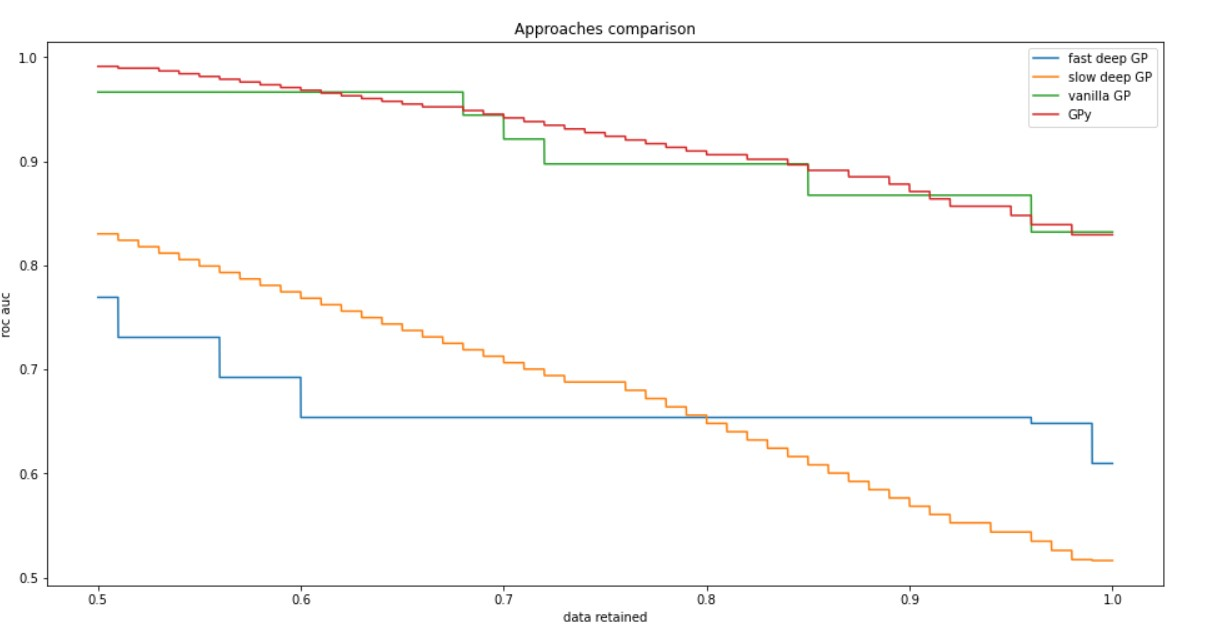
\includegraphics[width=\linewidth]{roc_auc.jpg}
\end{frame}

\begin{frame}{Текущие результаты}
На данный момент предложенные модели проигрывают уже существующим по критерию AUC. Предлагается выяснить причину такого расхождения и устранить ее, если возможно. 
\end{frame}


\begin{frame}{Продолжение работы}
\begin{enumerate}
    \item
	Добиться улучшения результатов работы сети.
	\item 
	Реализовать эффективное сэмплирование
	\item
	Исследовать подходы к поиску оптимальной подвыборки (BALD)
\end{enumerate}
\end{frame}

% \begin{frame}{Ссылки}
% \begin{block}
% Исследовательская группа М.Е. Панова
% \end{block}
% \end{frame}
%*********************************************************************************
\end{document} 
